\documentclass{beamer}

\usepackage[utf8x]{inputenc}
\usepackage{default}
\usepackage[italian]{babel}
\usepackage{graphicx}
\usepackage{textcomp} %per fare le frecce nel testo

\renewcommand{\thefootnote}{} %elimina il numerino della nota a piè di pagina
\renewcommand\footnoterule{} %elimina la riga prima della nota a piè di pagina

\usetheme{Warsaw}        % layout complessivo. 
\useinnertheme{default} % layout interno.
\useoutertheme{default} % layout esterno.
\usecolortheme{wolverine} % schema di colori.
\usefonttheme{default}  % schema dei font.

\hypersetup{pdfauthor={Ilario Gelmetti},pdfsubject={Chiralità ed amplificazione di chiralità in polimeri supramolecolari - Chirality in supramolecular polymers},pdfkeywords={chirality, chiral, polymers, supramolecular, amplification},pdftitle={Chiralita' ed amplificazione di chiralita' in polimeri supramolecolari}} %metadati nel pdf

\setbeamertemplate{navigation symbols}{} %per eliminare i bottoni della barra di navigazione in basso a destra

\AtBeginSection[]{\frame{\tableofcontents[current,hideothersubsections]}} %indice all'inizio di ogni section, mostra solo le sottosezioni di quella sezione

\title[Chiralità in polimeri supramolecolari]{Chiralità ed amplificazione di chiralità\\ in polimeri supramolecolari}
\subtitle{Esame di Complementi di Chimica Organica}
\author{Ilario Gelmetti}
\institute{Scuola Normale Superiore di Pisa.\\Professore Lorenzo Di Bari.}
\date{27 ottobre 2011}
\logo{
\includegraphics[width=0.07\paperwidth]{snslogo.png}}

\begin{document}
\begin{frame}
  \titlepage
\end{frame}

\section{Polimerizzazione supramolecolare}
\subsection{Polimeri supramolecolari}\begin{frame}\frametitle{Polimeri supramolecolari}
          \vspace{-5pt}  \begin{columns}
\column{0.6\linewidth}   \begin{definition}
              {\bf Supramolecular polymers} are defined as polymeric arrays of monomeric units that are {\bf brought together by reversible and highly directional secondary interactions}, resulting in polymeric properties in dilute and concentrated solution as well as in the bulk. \cite{12}
              \end{definition}\column{0.5\linewidth}
Le interazioni secondarie possono essere:
 \begin{itemize}
  \item legami ad idrogeno;
  \item interazioni di stacking $\pi-\pi$;
  \item interazioni idrofobiche;
  \item legami metallo-legante.
 \end{itemize}\end{columns}\vspace{10pt}
La polimerizzazione è un equilibrio, dunque \textbf{tutto è sotto controllo termodinamico}. Il grado di polimerizzazione del polimero non è stabile a variazioni di temperatura e concentrazione.
\end{frame}




\logo{}

\subsection{Meccanismi di polimerizzazione}\begin{frame}\frametitle{Meccanismi di polimerizzazione}
 \begin{columns}
\column{0.6\linewidth}\begin{itemize}
                       \item Pol. \textbf{isodesmica}: formazione di legami indipendentemente dal polimero, simile a pol. a stadi, alte polidispersità.
                       \item Pol. anello-catena: a basse conc. più anelli, ad alte conc. più catene.
                       \item Pol. \textbf{cooperativa}.
                       \end{itemize}
\column{0.5\linewidth}\vspace{-15pt}\begin{figure}{\centering{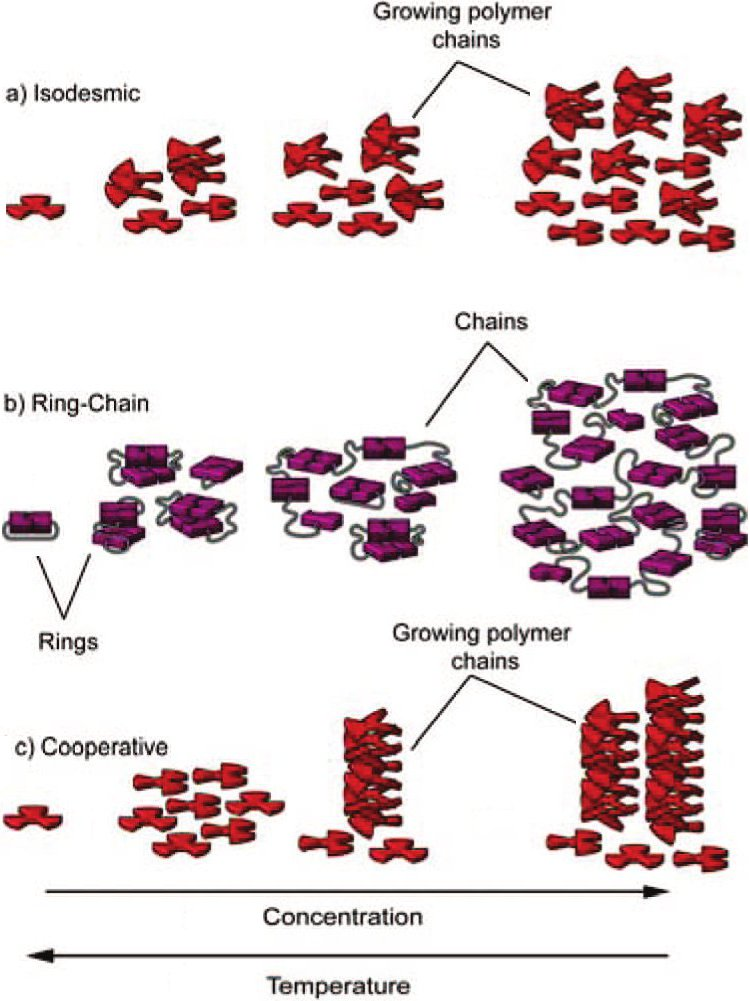
\includegraphics[width=1\textwidth]{sec0/polimerizzazione.jpg}}}\end{figure}\end{columns}
\end{frame}



\subsubsection{Polimerizzazione cooperativa}\begin{frame}\frametitle{Meccanismi di polimerizzazione}\framesubtitle{Polimerizzazione cooperativa}
\begin{columns}
\column{0.7\linewidth}La pol. \textbf{cooperativa} può essere \textbf{nucleata} (figura in alto) o \textbf{downhill} (in basso) o \textbf{anticooperativa} (basse polidispersità). 

Dall'oligomero si passa a polimero a lunga catena passando un punto critico
. Dipende dalla concentrazione, dalla temperatura ed eventualmente dall'eccesso enantiomerico.\column{0.3\linewidth}\vspace{-10pt}\begin{figure}{\centering{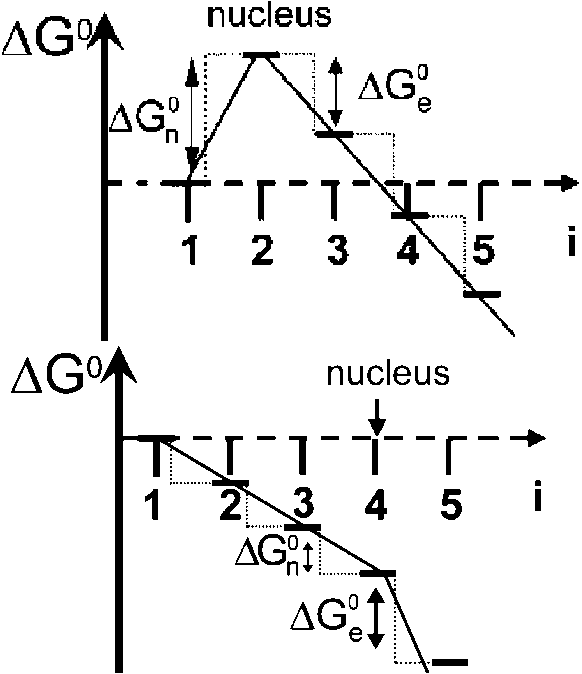
\includegraphics[width=0.9\textwidth]{sec0/cooperativa-2.png}}}\end{figure}
\end{columns}
 \begin{columns}
\column{0.35\linewidth}\begin{figure}{\centering{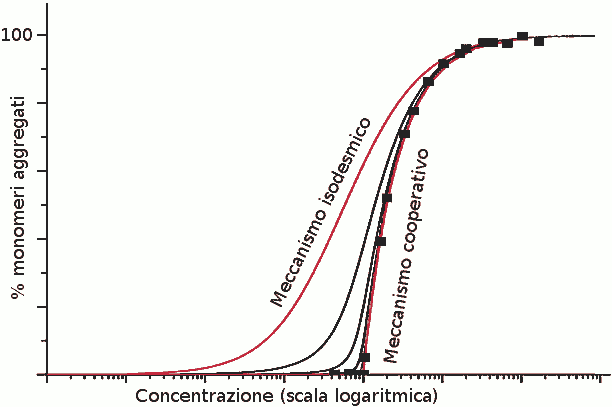
\includegraphics[width=1\textwidth]{sec0/conc.png}}}\end{figure}\column{0.65\linewidth}\begin{figure}{\centering{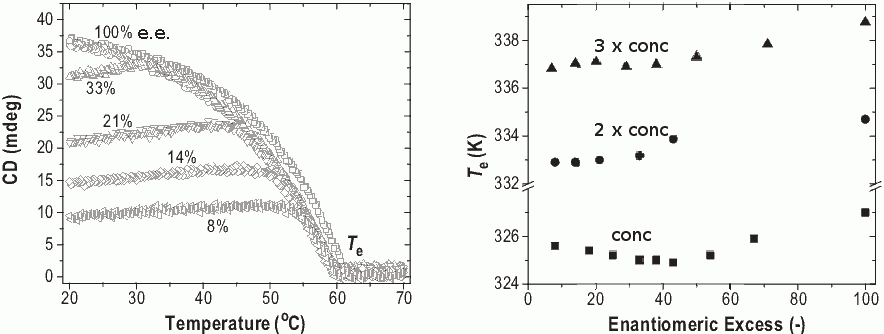
\includegraphics[width=1\textwidth]{sec0/temp_ee.png}}}\end{figure}
\end{columns}
\end{frame}\logo{
\includegraphics[width=0.07\paperwidth]{snslogo.png}}

\section{Amplificazione di chiralità}
\subsection{Chiralità in polimeri}\begin{frame}\frametitle{Chiralità in polimeri}
In polimeri con conformazione elicoidale si avranno {\bf regioni con rotazione destra o sinistra in equilibrio tra loro}; queste regioni saranno più lunghe se c'è alta energia di inversione. L'equilibrio può essere spostato con solventi chirali o chiralità sulle catene laterali.
\begin{columns}
\column{0.6\linewidth}In alcuni polimeri covalenti si ha una non-linearità dell'ellitticità con l'e.e. delle catene laterali. \cite{green}
\column{0.15\linewidth}\begin{figure}{\centering{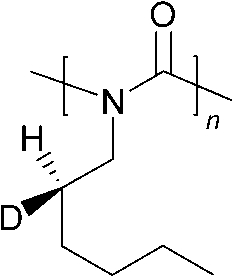
\includegraphics[width=1\textwidth]{sec1/polimero.png}}}\end{figure}\end{columns}\vspace{10pt}
\textbf{A differenza delle reazioni} in cui si ha amplificazione di chiralità qui \textbf{non aumenta l'e.e.} bensì aumenta la \textbf{chiralità osservabile}.

             \end{frame}
\subsection{Amplificazione di chiralità}
\subsubsection{Penalità nell'energia}\begin{frame}\frametitle{Amplificazione di chiralità}\framesubtitle{Penalità nell'energia}

I modelli utilizzati per l'amplificazione di chiralità considerano due contributi energetici:
\begin{itemize}
 \item penalità per {\bf inversione di elica}. \emph{Helix reversal penality: penalizes a helix reversal along the chain. It is invoked when two consecutive bonds have different conformations.}

 \item Penalità per {\bf errore puntuale}. \emph{Mismatch penality: penalizes a mismatch between the preferred screw sense of a monomer and the bonds near to it. It is used
whenever a “+” bond follows or precedes a “-” monomer, and vice versa. We apply the mismatch penalty twice when both monomers surrounding a bond are of the type incompatible with that bond.  }\cite{def}
\end{itemize}
\end{frame}
\subsubsection{Sergenti e soldati}\begin{frame}\frametitle{Amplificazione di chiralità}\framesubtitle{Sergenti e soldati}
Per valutare la non-linearità si possono misurare due effetti:

{\bf Sergenti e soldati}: tra molte unità monomeriche achirali poche unità chirali dirigono la chiralità della conformazione polimerica.

\begin{figure}{\centering{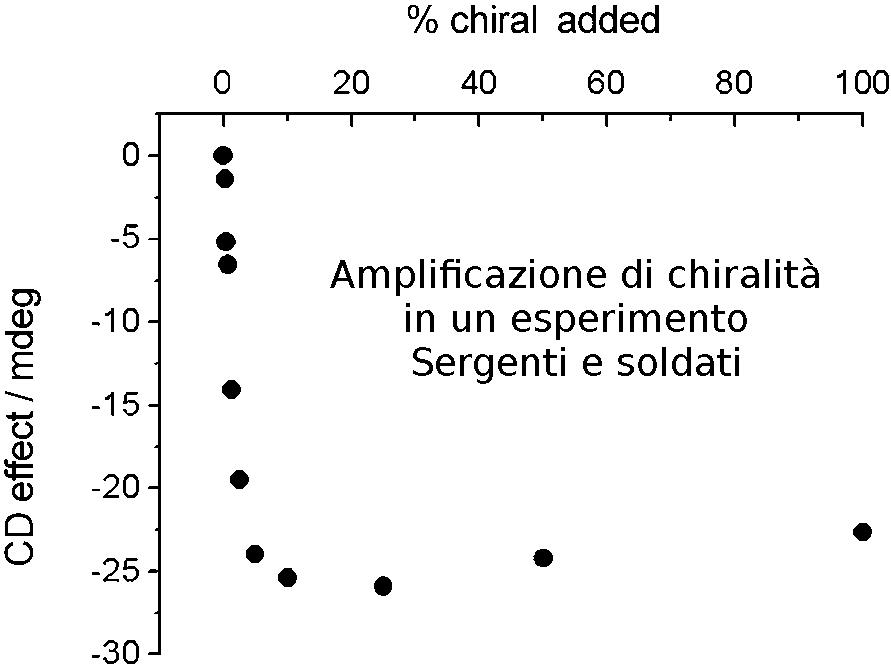
\includegraphics[width=0.5\textwidth]{sec1/sergenti.png}}}\end{figure}
\end{frame}

\subsubsection{Regola di maggioranza}\begin{frame}\frametitle{Amplificazione di chiralità}\framesubtitle{Regola di maggioranza}
{\bf Regola di maggioranza}: la conformazione di una catena con entrambi i monomeri enantiomerici viene dettata da quello in maggioranza. Avviene quando la penalità per errore puntuale 
 è inferiore alla penalità per inversione di elica.

\begin{figure}{\centering{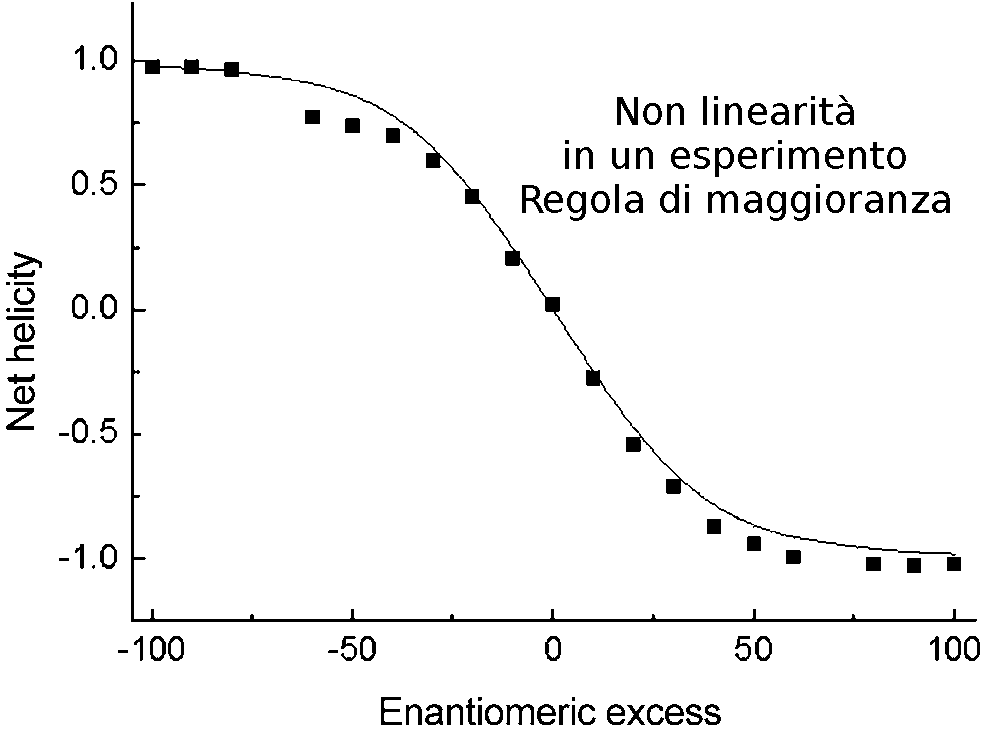
\includegraphics[width=0.4\textwidth]{sec1/maggioranza.png}}}\end{figure}
\end{frame}


\section{Aggregazione di unità discotiche}
\subsection{Unità con simmetria $C_3$}\begin{frame}\frametitle{Unità con simmetria $C_3$}
  \vspace{-5pt}   \begin{columns}
\column{0.3\linewidth}    \begin{figure}{\centering{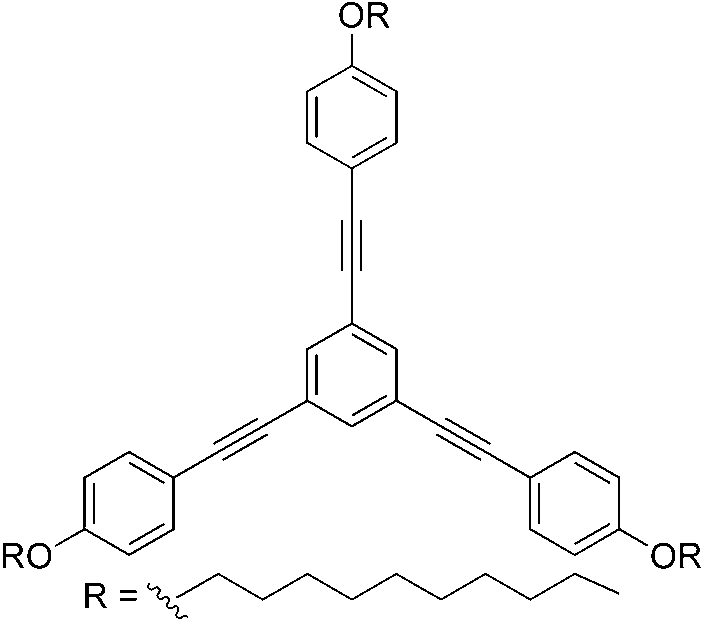
\includegraphics[width=0.8\textwidth]{sec2/alchino.png}}}\end{figure}    \column{0.3\linewidth} 
\begin{figure}{\centering{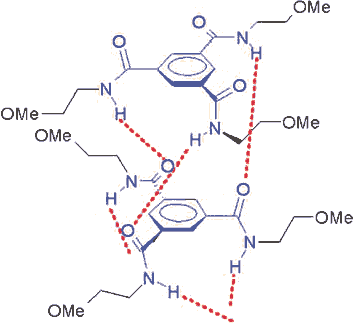
\includegraphics[width=0.8\textwidth]{sec2/C3legami.png}}}\end{figure}
 \column{0.3\linewidth} 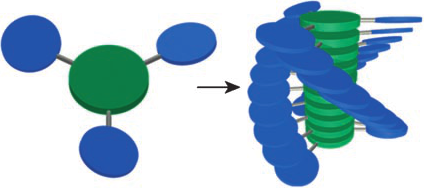
\includegraphics[width=1\textwidth]{sec2/C3.png}\end{columns}\vspace{15pt}
 
La conformazione elicoidale può esser causata da ingombro sterico (molecola a sinistra) o da nuovi legami ad idrogeno intermolecolari (molecola al centro). 


Variando le interazioni direzionali è possibile ottenere elicità controllate.

È \textbf{importante il bilancio delle interazioni}: 
troppe adirezionali diminuiscono l'ordinamento chirale indotto dalle direzionali.
             \end{frame}\logo{}
\subsection{Cooperatività}\begin{frame}\frametitle{Cooperatività}
   \begin{columns} \column{0.4\linewidth}La prima polimerizza cooperativamente.\begin{figure}{\centering{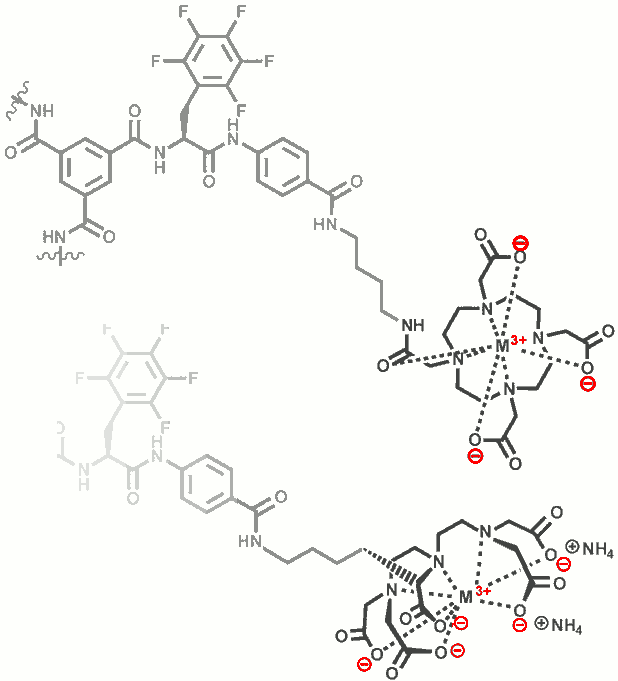
\includegraphics[width=1\textwidth]{sec2/anticoop.png}}}\end{figure} \column{0.6\linewidth} La motivazione è la presenza \textbf{nel dimero} dei \textbf{gruppi ammidici già orientati correttamente}.             \cite{tesi}
\begin{figure}{\centering{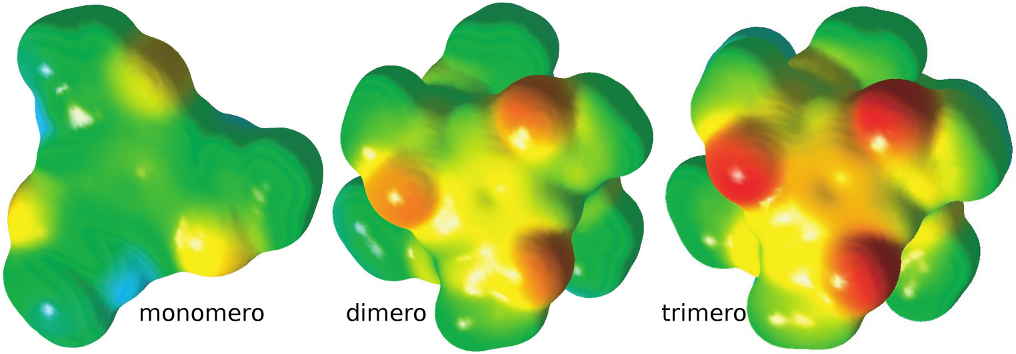
\includegraphics[width=0.7\textwidth]{sec2/1-2.png}}}\end{figure}
La seconda molecola ha polimerizzazione anticooperativa (controllo della dimensione). Alzando la forza ionica della soluzione diventa cooperativa. \cite{2}\end{columns}            
                                      \end{frame}\logo{
\includegraphics[width=0.07\paperwidth]{snslogo.png}}
\subsection{Amplificazione di chiralità}\subsubsection{Catene laterali}\begin{frame}\frametitle{Amplificazione di chiralità}\framesubtitle{Catene laterali}
L'interazione sterica tra catene laterali chirali può indurre un senso di rotazione preferenziale. \textbf{I monomeri non hanno CD} perciò misurazioni CD sono sensibili solo alla chiralità supramolecolare.\vspace{10pt}
\begin{columns}
\column{0.8\linewidth} \textbf{Effetto pari-dispari}: spostando di un carbonio il centro chirale si ha una inversione dei segni dei picchi al CD mantenendo lo stesso modulo, dunque un'inversione di rotazione dell'aggregato.\column{0.2\linewidth}\vspace{-20pt}\begin{figure}{\centering{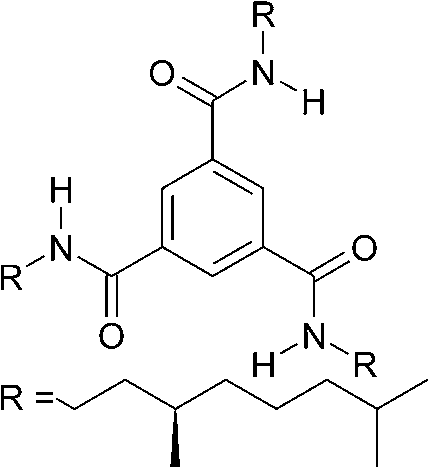
\includegraphics[width=1\textwidth]{sec2/C3semplice.png}}}\end{figure}\end{columns}\vspace{10pt} % \vspace{20pt}
\textbf{Se delle tre catene laterali solo una è chirale}, l'ellitticità in un omopolimero non varia. Invece la \textbf{penalità per errore puntuale diminuisce} (dunque l'ampl. chirale in esp. sergenti e soldati diminuisce ma aumenta in esp. regola di maggioranza). \cite{tesi}
\end{frame}
\logo{}
\subsubsection{Effetto della temperatura}\begin{frame}\frametitle{Amplificazione di chiralità}\framesubtitle{Effetto della temperatura}
L'\textbf{aumento della temperatura} provoca: \cite{tesi}
\begin{itemize}
 \item pol. omochirale CD\textdownarrow (a causa della \textbf{disaggregazione});\\ ellitticità molare -- (si riferisce solo alla frazione aggregata);
\end{itemize}
\begin{columns}
\column{0.6\linewidth}
\begin{itemize}
 \item penalità per inversione -- ( \textdownarrow poco,\\ è correlata ai legami ad idrogeno e questi restano intatti);
 \item penalità per errore \textdownarrow ;
 \item sergenti e soldati \textdownarrow (\textdownarrow la capacità di imporre chiralità);
 \item regola di maggioranza \textuparrow .
\end{itemize}

Scaldando ulteriormente si ha completa solubilizzazione molecolare.
\column{0.5\linewidth}\begin{figure}{\centering{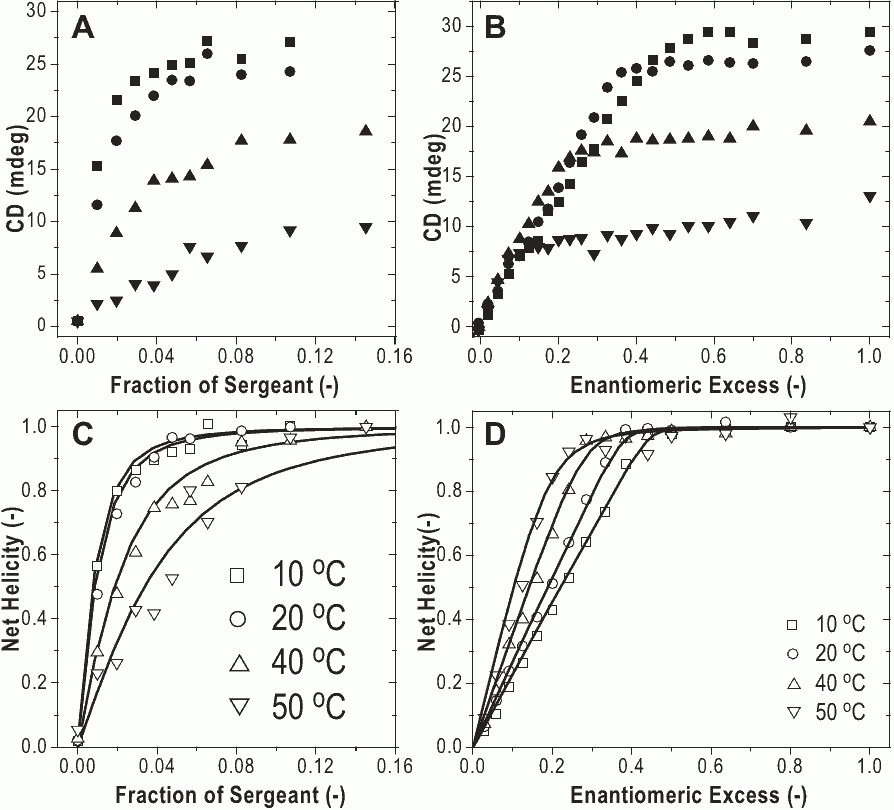
\includegraphics[width=1\textwidth]{sec2/temp.png}}}\end{figure}\end{columns}
\end{frame}


\subsubsection{Regola di maggioranza}\begin{frame}\frametitle{Amplificazione di chiralità}\framesubtitle{Regola di maggioranza}
\begin{columns}
\column{0.64\linewidth}\textbf{Per avere una maggiore amplificazione chirale in esp. regola di maggioranza} si può diminuire la \textbf{penalità per errore} ma non troppo: esiste un valore \textbf{ottimale}. Infatti una penalità=0 significherebbe che la chiralità non viene più espressa ad un livello supramolecolare.

Con un valore \textbf{maggiore della penalità per inversione} di elica si ha un valore minore dell'ottimo di penalità per errore ed un \textbf{minore e.e. a cui si avrà omochiralità} supramolecolare. \cite{tesi}
\column{0.36\linewidth}\vspace{-13pt}
\begin{figure}{\centering{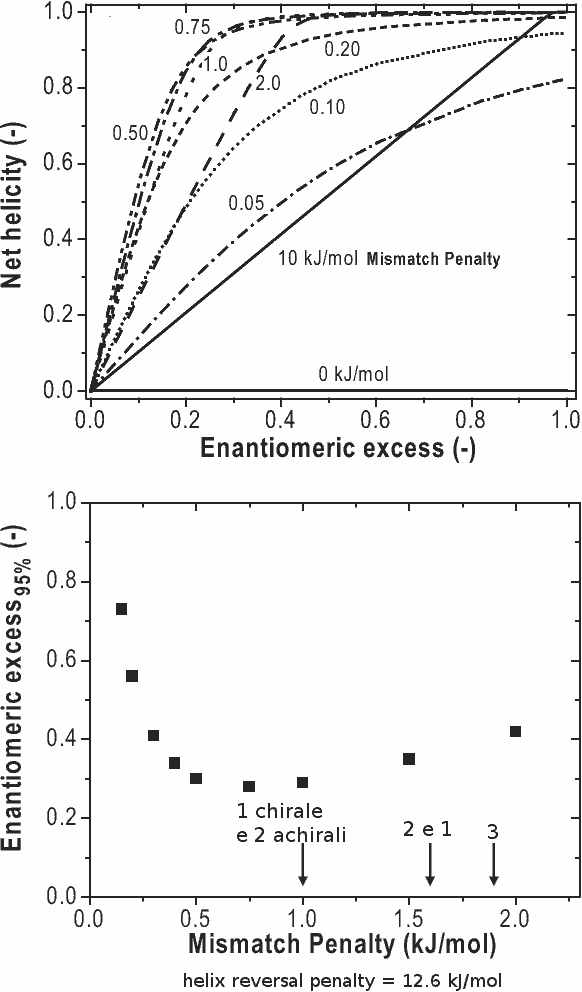
\includegraphics[width=1\textwidth]{sec2/maggioranza-ottimo.png}}}\end{figure}
\end{columns}
\end{frame}
\logo{
\includegraphics[width=0.07\paperwidth]{snslogo.png}}

\subsection{Altre unità discotiche}\begin{frame}\frametitle{Altre unità discotiche}
\begin{columns}
\column{0.4\linewidth}
\begin{figure}{\centering{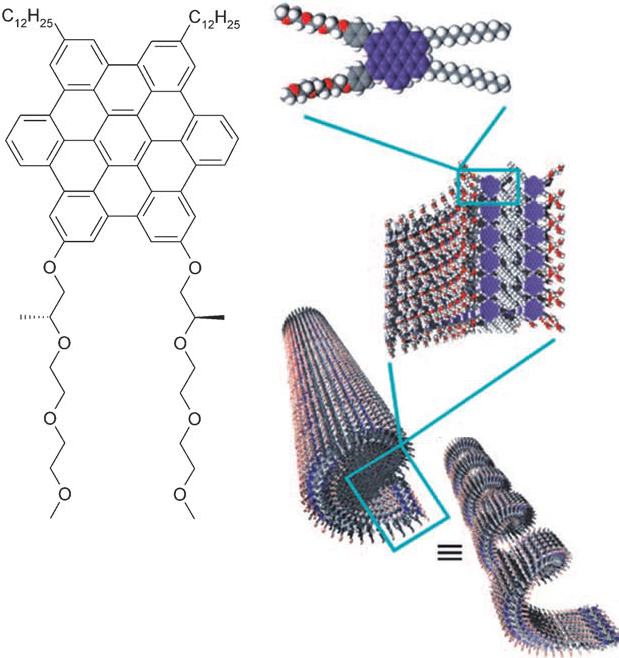
\includegraphics[width=1\textwidth]{sec2/coronene.png}}}\end{figure}
Forte \textbf{amplificazione} di chiralità.
\column{0.6\linewidth}\begin{columns}
\column{0.6\linewidth}
\begin{figure}{\centering{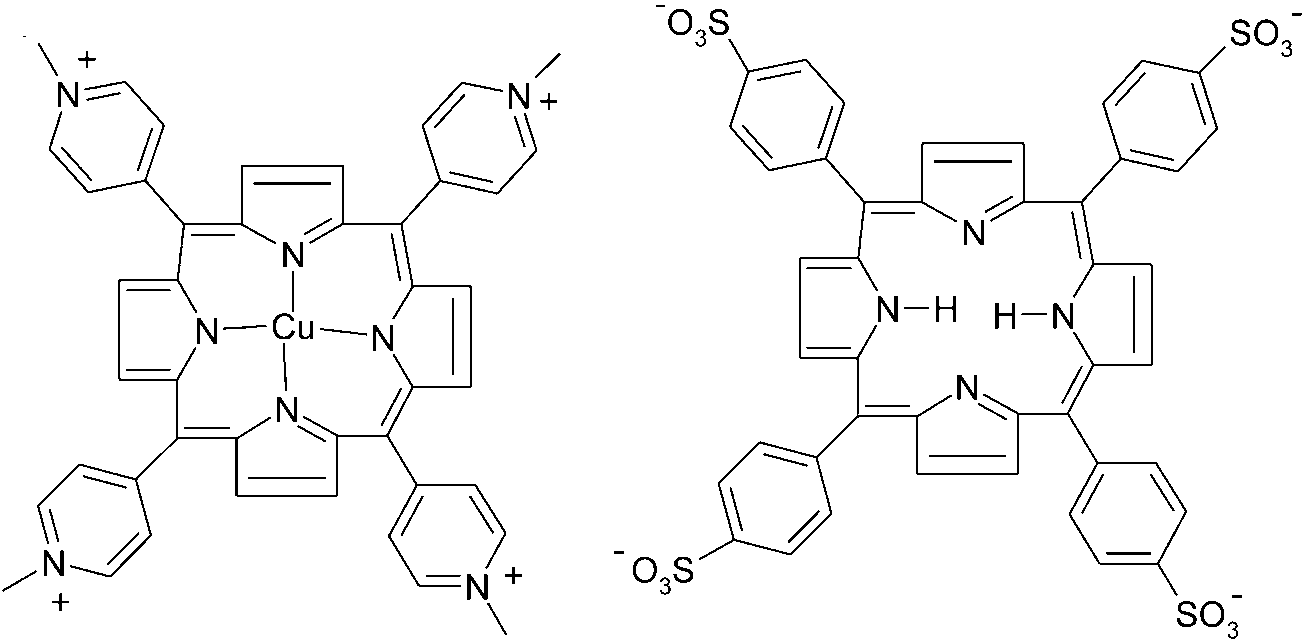
\includegraphics[width=1\textwidth]{sec2/porfirine.png}}}\end{figure}
\column{0.4\linewidth}Spontaneamente in eliche, \textbf{memorizzano la chiralità} dal templato di poliglutammato.\end{columns}
\begin{columns}
\column{0.6\linewidth}\begin{figure}{\centering{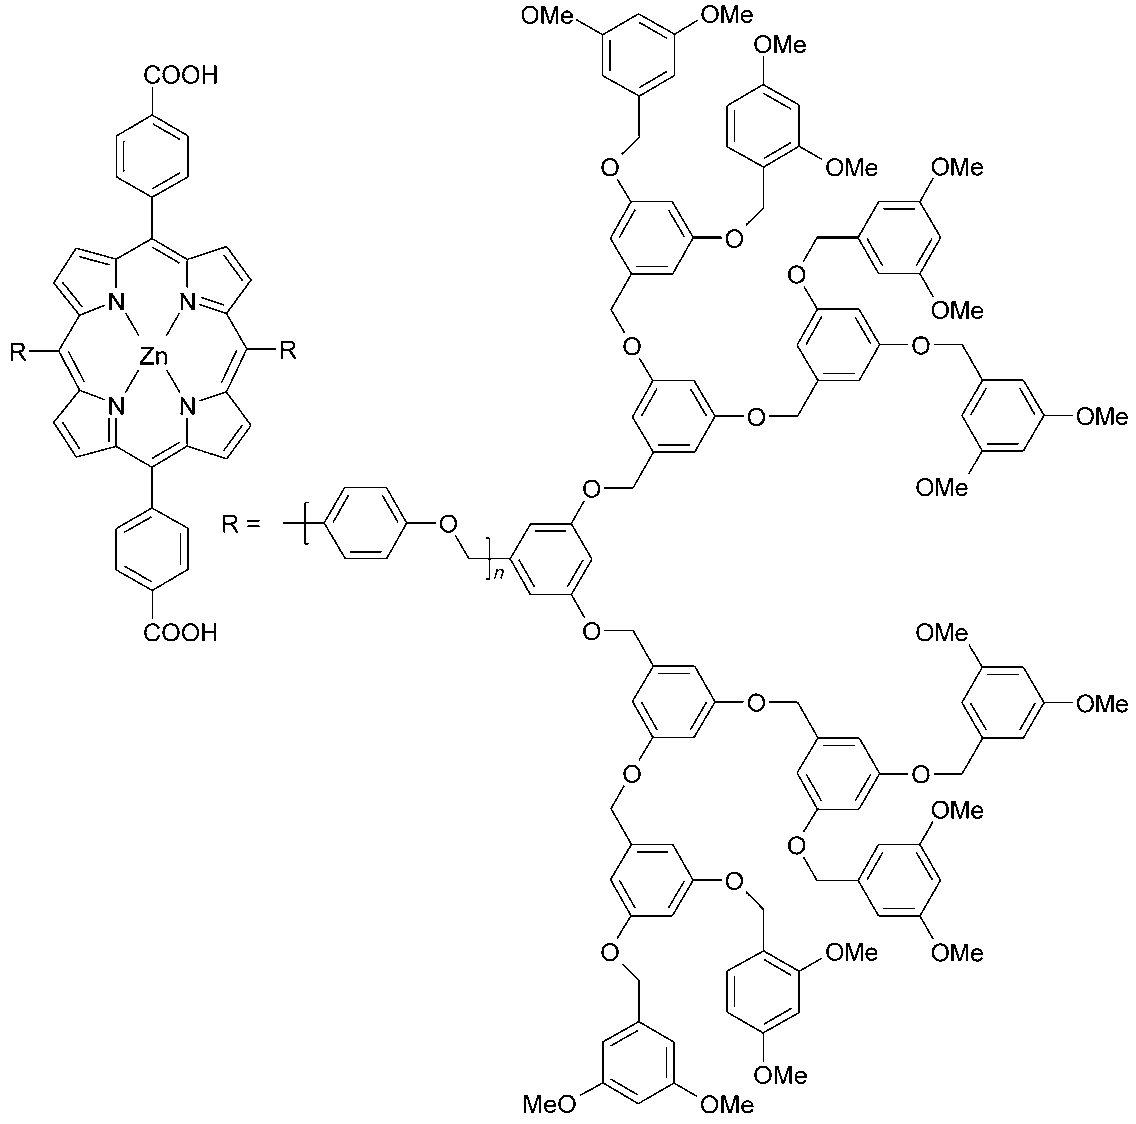
\includegraphics[width=1\textwidth]{sec2/zinco-dendritico.png}}}\end{figure}\column{0.4\linewidth}
Induzione di chiralità dalla \textbf{direzione dello spin-coating}.
\end{columns}\end{columns}
\end{frame}

\section{Aggregazione di unità allungate e polimeri}
\subsection{Unità monomeriche}\subsubsection{Aggregazione per legami ad idrogeno}\begin{frame}\frametitle{Unità monomeriche}\framesubtitle{Aggregazione per legami ad idrogeno}
\begin{columns}
\column{0.25\linewidth}  \vspace{-5pt}  \begin{figure}{\centering{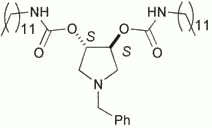
\includegraphics[width=1\textwidth]{sec3/carbammato.png}}}\end{figure}\vspace{-10pt}\begin{figure}{\centering{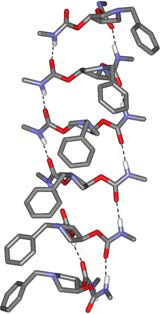
\includegraphics[width=0.8\textwidth]{sec3/carbammato-conformazione.png}}}\end{figure}
\column{0.75\linewidth} 
Il \textbf{monomero} in figura (con il cromoforo fenilico lontano dal centro chirale $\Rightarrow$ \textbf{non ha CD}) da aggregazione in strutture elicoidali.

I cromofori possono presentare \textbf{accoppiamento eccitonico} e dunque un CD indicativo dell'orientazione relativa. 

Gli aggregati danno fibre con avvolgimento osservabile tramite microscopia.

Si osserva \textbf{linearità} in esp. regola di maggioranza, avviene una \textbf{discriminazione enantiomerica} ossia una segregazione in \textbf{2 fibre} enantiomericamente \textbf{pure}. \cite{4}
\end{columns}
  \end{frame} 

\subsubsection{Aggregazione per interazione idrofobica}\begin{frame}\frametitle{Unità monomeriche}\framesubtitle{Aggregazione per interazione idrofobica}
\vspace{-5pt}\begin{columns}
\column{0.6\linewidth}\begin{figure}{\centering{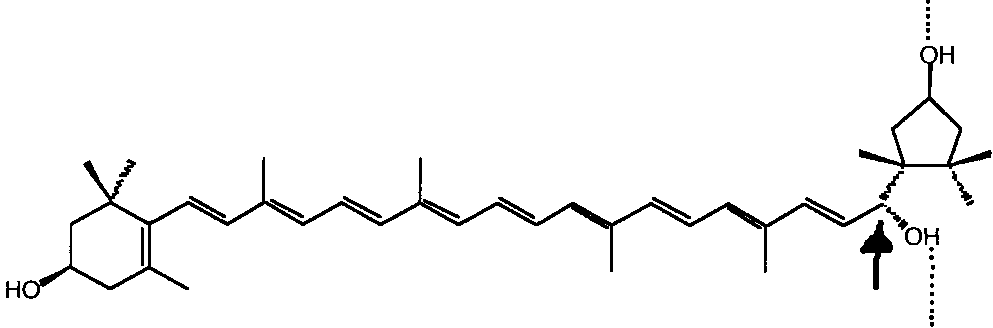
\includegraphics[width=0.8\textwidth]{sec3/carotenoide.png}}}\end{figure}\column{0.4\linewidth}\begin{figure}{\centering{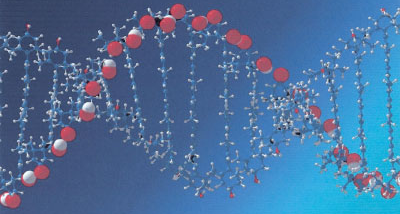
\includegraphics[width=0.9\textwidth]{sec3/carotenoide3d.png}}}\end{figure}\end{columns}
\vspace{10pt}
L'aggregazione avviene per \textbf{interazione idrofobica}, anche qui al CD si osserva l'accoppiamento eccitonico. 

A seconda della configurazione del carbonio indicato si possono avere \textbf{aggregati supramolecolari di tipo J o di tipo H} (J~=~aggregazione debole (testa-coda) e red shift dell'assorbimento; H~=~aggregazione compatta e blue shift). 

In figura l'aggregazione di tipo H in cui si ha una catena di legami ad idrogeno (evidenziati nelle figure). \cite{9}
  \end{frame} 

\subsection{Unità oligomeriche}\begin{frame}\frametitle{Unità oligomeriche}
           \begin{columns}
\column{0.5\linewidth}\begin{figure}{\centering{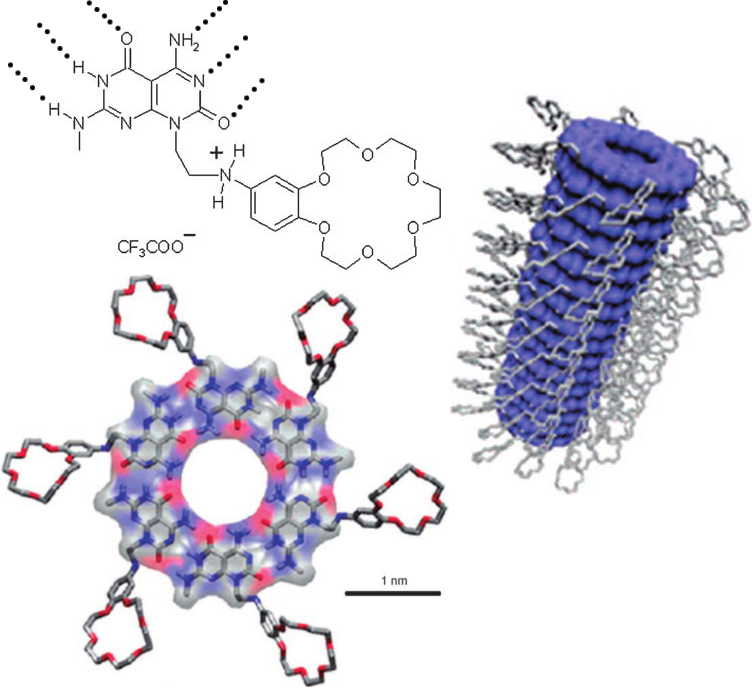
\includegraphics[width=1\textwidth]{sec3/oligomeri.png}}}\end{figure}\column{0.5\linewidth}   Il monomero \textbf{achirale} si assembla in dischi grazie ai legami ad idrogeno, dunque si aggrega in nanotubi. 

La \textbf{chiralità} viene \textbf{indotta} in modo non-lineare (cooperativa) aggiungendo un \textbf{amminoacido} chirale. \cite{8}
       \end{columns}      \end{frame}  

      \subsection{Unità polimeriche}\begin{frame}\frametitle{Unità polimeriche}
              \begin{columns}
\column{0.3\linewidth}\begin{figure}{\centering{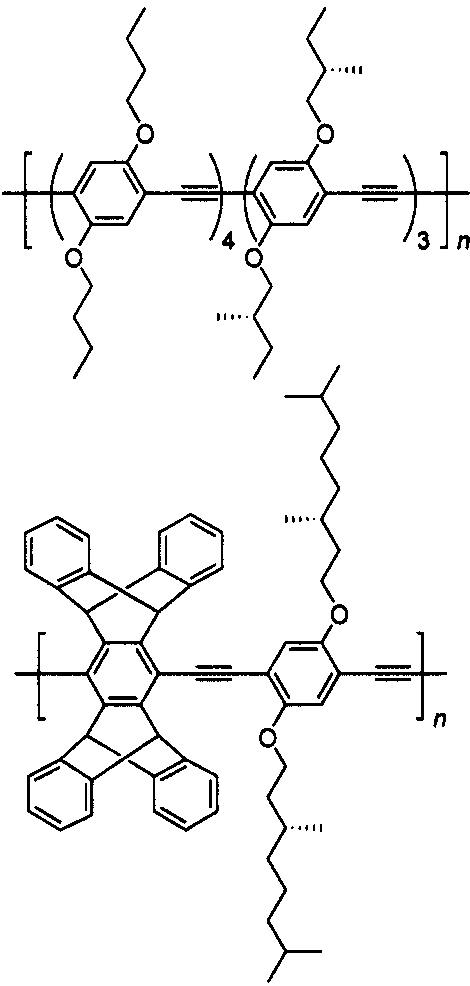
\includegraphics[width=0.9\textwidth]{sec3/polimeri.png}}}\end{figure}\column{0.7\linewidth} Utilizzare polimeri con della chiralità permette di \textbf{studiarne la conformazione utilizzando il CD} e di \textbf{impedire la formazione di aggregati allineati} allo scopo di ottenere proprietà optoelettroniche diverse (evitare il quenching di fluorescenza mantenendo l'accoppiamento elettronico intercatena). \cite{1} \end{columns}    
             \end{frame}    



\setbeamertemplate{bibliography item}[text] %nella bibliografia in fondo ci mette i numeri invece del simbolo inutile del documento
\begin{frame}[plain
]
{\tiny{\bibliographystyle{apalike}
\bibliography{bib/compl_chim_org.bib}
}}
\end{frame}


\end{document}
